%!TEX program = xelatex
%!TEX TS-program = xelatex
%!TEX encoding = UTF-8 Unicode

\documentclass[12pt, a4paper]{article}
\usepackage{CJKutf8}
\usepackage{graphicx}
\usepackage{subfigure}
\usepackage{listings}
\usepackage[colorlinks,linkcolor=blue]{hyperref}
\usepackage{ulem}
\usepackage{xcolor}
\usepackage{caption2}
\usepackage{amssymb}
\usepackage{indentfirst} % 中文段落首行缩进
\setlength{\parskip}{0.5em}
\renewcommand{\figurename}{图} % 将图表的标题设置为中文“图”

\title{第十七·重复博弈·制定策略考虑长远影响}
\author{hoochanlon}
\date{\today}

\begin{document}
	\begin{CJK*}{UTF8}{gbsn}
		\maketitle
        \clearpage
        \section{重复博弈的概念及特征}
        \subsection{重复博弈的三个概念}
        \begin{enumerate}
            \item 同样的结构的博弈结构重复很多次。
            \item 其中的每次博弈称为“阶段博弈”。
            \item 可以是完全信息的,也可以是不完全信息的。
        \end{enumerate}
        当博弈只进行一次的时候,每个参与人他只关心当下的收益,如果博弈是重复很多次的,那么参与人可能就会为了长远利益,牺牲眼前利益。
        \subsection{重复博弈的三个基本特征}
        \begin{enumerate}
            \item 重复博弈中各阶段博弈之间没有“物质”上的联系,即前一个阶段博弈并不改变后一个阶段的博弈结构。
            \item 在重复博弈的每一个阶段,所有参与人都观测到该博弈所有过去的历史。(条件、规则、内容相同)
            \item 参与人的总损益是所有阶段博弈损益的贴现值之和。
        \end{enumerate}
        由于有长期利益的存在,各个参与者在当前阶段博弈中,就需要考虑不能引起其他参与者在后面阶段的对抗、报复。所以每一个参与者不能像静态博弈中,
        毫不顾忌的根本不顾及他人的利益而抉择,所以一方做出一种合作的行动,他会使其他参与者在后面阶段也参与合作的这样的行动,从而实现更长期、更大的利益。 \par

        重复博弈的最大贡献:对人们之间的合作行为,提供一个基于个人理性的解释。囚犯困境博弈一次性的唯一均衡解,大家都不合作,都选择坦白。
        但如果是重复博弈,合作的行为就有可能了。在这里需强调,重复博弈中必须考虑对方的利益而选择(非利他主义,而是出于对自身长远利益的考虑)。

        \clearpage
        \section{重复博弈:以囚犯困境为例}
        不难看出双方合作肯定是最好的,但在一次性博弈中,双方的占优策略是各自都背叛,所以构成了占优策略的纳什均衡。

        \begin{figure}[htbp]
            \centering
            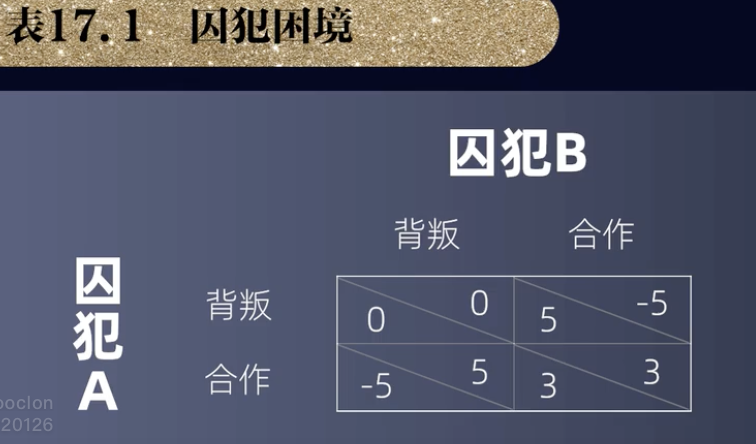
\includegraphics[width=0.6\textwidth]{./figures/catch2023-08-02-09.08.38.png}
            \caption{囚犯困境模型}
        \end{figure}

        如果博弈不是一次性的,有更多重复,那么这个时候每个参与者就有了更多的策略选择。

        \section{可选择的策略}

        \subsection{可选策略 v1.0}
        在无限次的重复博弈中,其实每个参与者,他是有无穷数量的策略选择的。
        \begin{enumerate}
            \item 好人策略:无论对方如何选择,每次都选择合作。(烂好人)
            \item 曹操策略:无论对方如何选择,每次都选择背叛。(宁可我负天下人,休教天下人负我)
            \item 冷酷策略:又叫触发策略,首次选择合作合作只要对方合作,就一直选择合作,一旦对方选择背叛,则永远选择背叛。(一次不忠,百次不用,绝无机会)
            \item 心太软策略:首次选择合作,可以接受对方一次背叛,一旦对方连续两次背叛就永远背叛,坏处就是老是给对方机会。
            \item 一报还一报策略:第一次选择合作,以后每次都选择对方上一次的选择。(合作的人我也合作,背叛的人我也背叛)
        \end{enumerate}

        \subsection{可选策略 v2.0}
        就是千万不要被别人误以为你是醉汉,否则的话没有人会对你好的。
        \begin{enumerate}
            \item 道宁策略:第一步背叛,然后每走一步,估计对方合作的概率,如果对方似乎仍然倾向于合作,则选择背叛;反之选择合作。(欺软怕硬)
            \item 乔斯策略:试图偶尔背叛而不受惩罚。对方合作10次以后,随机选择一次作为背叛的试探。(老是像占便宜)
            \item 醉汉策略:随机合作,随机背叛。
        \end{enumerate}

        \section{艾克斯罗德的贡献}
        \subsection{艾克斯罗德的竞赛}

        比赛规则:总博弈的次数是200次;双方合作各得3分;都背叛则各得1分;一方背叛,一方合作,背叛的一方得5分,合作的一方得0分。

        比赛结果:
        \begin{figure}[htbp]
            \centering
            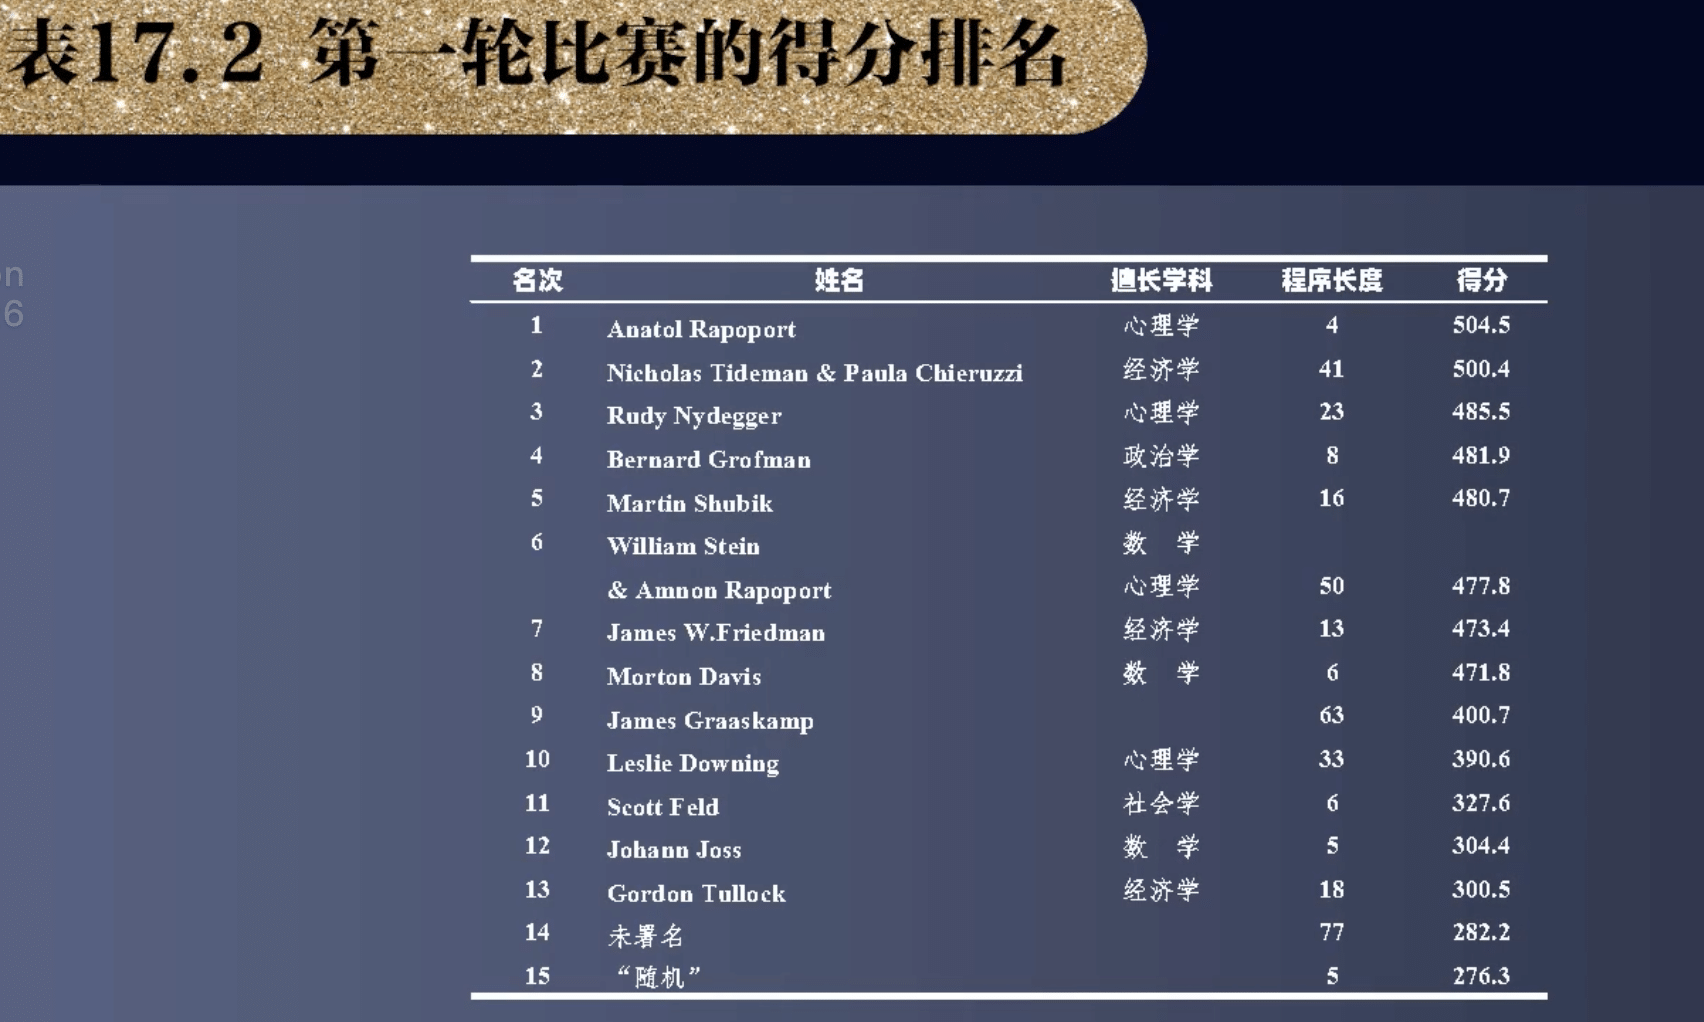
\includegraphics[width=1\textwidth]{./figures/catch2023-08-02-10.04.06.png}
            \caption{第一次比赛结果}
        \end{figure}

        新增策略:

        \begin{itemize}
            \item 一报还两报:仅当对手连续背叛两次以上,才选择背叛,其他与一报还一报相似。
            \item 检验者策略:第一步选择背叛,然后观察对方的态度。如果对方背叛,就改为按一报还一报行事;如果对方不背叛,则在2、3步合作,
            但以后没隔一步就背叛一次。(专门欺负软骨头)
            \item 哈灵顿策略:首先合作,当发现对方一直在合作,他就突然来个背叛,如果对方立刻报复它,它就恢复合作;如果对方仍然合作,它就继续背叛。
        \end{itemize}

        艾克斯罗德总结,“一报还一报”策略排名第一的原因:
        \begin{enumerate}
            \item 善良性:即不作首先的背叛者。
            \item 可激怒性:即应该针对对手的背叛行为给予报复。(预防用乔斯策略老是被占便宜)
            \item 宽容性:不因对方的一次背叛,就没完没了的报复。
            \item 清晰性:即策略简单,容易被辨识。
        \end{enumerate}
        针锋相对的善良性,防止陷入非合作的麻烦中,对对方背叛的报复,则保证了对方,背叛行为的谨慎性。宽容性,有助于在对方背叛以后,我们还能有机会合作。
        简单清晰的规则,易于被他人所理解,从而导出一个长期的合作关系。\par
        艾克斯罗德在《合作的进化》指出,一报还一报策略,它能社会各个领域的合作。包括在一些最无指望的环境中的合作。比如第一次世界大战,自发产生了“我自己活,也要让别人活”的原则。
        双方军队互相对峙好几个月,于是就有了各自互相适应的机会。

        \section{对冷酷策略的进一步分析}
        冷酷策略的核心理念:任何参与者的一次背叛将触发永远的背叛。冷酷策略不给对方任何改正错误的机会,如果对手是采取冷酷策略,最好的选择就是合作。
        这样的结果是无限次重复博弈中的所有参与者,因为他害怕冷酷策略的永远背叛,导致大家更容易出现合作关系。冷酷策略的外表,是有颗友善的内心。
        不过在艾克斯罗德竞赛中冷酷策略得分相当低,冷酷策略被辨识和验证成本太高,它的威胁也就不可置信。
        \textbf{在重复博弈中,最重要的目的不是惩罚对手,而是尽快建立合作关系,最好是建立一种稳固的合作关系。} \par

        一个采取冷酷策略的贴现因子,其实他并不能保证对手的永久合作,即背叛了你之后,背叛你收益高,对其他人的合作,还能持续赚收益。

        \section{一报还一报的策略启发}
        人生赢家的秘诀不在于赢过一个又一个对手,而在于是否能与各种各样的人建立起合作关系:一报还一报对各种不同策略适应性强,虽然不是相对应环境的策略,
        比如:面对好人策略、醉汉策略,最佳策略是曹操;面对心太软策略、最佳策略是tester检验者策略。当然很多这种看似随机应变、左右逢源,
        殊不知其实你看很多时候,我们认识和了解一个人的成本是相当高的。你以为是个好人,没想到他是个曹操,或者冷酷者。而且问题还在于参与者的策略也会进行动态调整,
        对于一报还一报而言,我不管你是谁,我只想让你知道我是谁。你只要知道我是一报还一报,那么我们就很容易建立起关系。合作的前提不是彼此信任,而是关系的持续性。\par

        重复博弈的核心,把未来的收益折算成眼前的利益,那么贴现因子越大,越看重未来利益。那么参与者他们往往就越愿意合作。当我们把贴现因子看成下次博弈的可能性,
        那么就意味着再次博弈的可能性越大,那么参与者选择合作的可能性就越大。人们之所以愿意合作,不是“你不相信我,我不相信你”,而是因为我们下次还要继续博弈,
        所以远亲不如近邻其实就是这个意思。另外,组织相对个人往往有更长的预期寿命,从而会提高我们关系的持续性。\par



    \end{CJK*}
\end{document}
